% 
% Lecture Template for ME3050 -  Dynamics Modeling and Controls - Tennessee Technological University
%
% Tristan Hill, May 07, 2020 - June 12, 2020, % Spring 2020 - Summer 2020
% Module 6 - Spring Systems
% Topic 1 - The Ideal Spring 
%

\documentclass{beamer}                         % for presentation (has nav buttons at bottom)
%\documentclass[handout]{beamer}  % for handout 
\usepackage{beamerthemesplit}
\usepackage{amsmath}
\usepackage{listings}
\usepackage{multicol}
\usepackage{framed}

\beamertemplateballitem

% custom colors
\definecolor{TTUpurple}{rgb}{0.3098, 0.1607, 0.5176} % TTU Purple (primary)
\definecolor{TTUgold}{rgb}{1.0000, 0.8666, 0.0000} % TTU Gold (primary) 
\definecolor{mygray}{rgb}{.6, .6, .6}
\definecolor{mypurple}{rgb}{0.6,0.1961,0.8}
\definecolor{mybrown}{rgb}{0.5451,0.2706,0.0745}
\definecolor{mygreen}{rgb}{0, .39, 0}
\definecolor{mypink}{rgb}{0.9960, 0, 0.9960}

% color commands
\newcommand{\R}{\color{red}}
\newcommand{\B}{\color{blue}}
\newcommand{\BR}{\color{mybrown}}
\newcommand{\K}{\color{black}}
\newcommand{\G}{\color{mygreen}}
\newcommand{\PR}{\color{mypurple}}
\newcommand{\PN}{\color{mypink}}
\newcommand{\OR}{\color{TTU}}
\newcommand{\GD}{\color{TTUgold}}

% beamer colors
\setbeamercolor{palette primary}{bg=TTUpurple,fg=TTUgold}
\setbeamercolor{palette secondary}{bg=black,fg=TTUgold}
\setbeamercolor{palette tertiary}{bg=black,fg=TTUpurple}
\setbeamercolor{palette quaternary}{bg=TTUgold,fg=black}
\setbeamercolor{structure}{fg=TTUpurple} % itemize, enumerate, etc
\setbeamercolor{section in toc}{fg=TTUpurple} % TOC sections


\newcommand{\Lagr}{\mathcal{L}} % lagrangian

\newcommand{\hspcu}{\underline{\hspace{20mm}}} % large horizontal space w underline
\newcommand{\vspccc}{\vspace{6mm}\\} % large vertical space
\newcommand{\vspcc}{\vspace{4mm}\\}   % medium vertical space
\newcommand{\vspc}{\vspace{2mm}\\}     % small vertical space

\newcommand{\hspcccc}{\hspace{10mm}} % large horizontal space
\newcommand{\hspccc}{\hspace{6mm}} % large horizontal space
\newcommand{\hspcc}{\hspace{4mm}}   % medium horizontal space
\newcommand{\hspc}{\hspace{2mm}}     % small horizontal space

\newcommand{\eqscl}{0.9}     % small horizontal space

\newsavebox{\mybox} % custom box


\newcommand{\MNUM}{5\hspace{2mm}} % Module number
\newcommand{\TNUM}{1\hspace{2mm}} % Topic number 
\newcommand{\moduletitle}{Spring Systems} % Titles and Stuff
\newcommand{\topictitle}{The Ideal Spring} 

\newcommand{\sectiontitleI}{Robert Hooke} % More Titles and Stuff
\newcommand{\sectiontitleII}{Hooke's law of Springs}
\newcommand{\sectiontitleIII}{The Spring Model}
\newcommand{\sectiontitleIV}{Structure Stiffness}

\author{ME3050 - Dynamics Modeling and Controls}
\title{Module \MNUM - \moduletitle}
\date{Mechanical Engineering\vspc Tennessee Technological University}

\begin{document}

\lstset{language=MATLAB,basicstyle=\ttfamily\small,showstringspaces=false}

\frame{\titlepage \center\begin{framed}\Large \textbf{Topic \TNUM - \topictitle}\end{framed} \vspace{5mm}}

% Section 0 - Outline
\frame{
	
	\large \textbf{Topic \TNUM - \topictitle} \vspace{3mm}\\
	
	\begin{itemize}
	
		\item \sectiontitleI    \vspc % Section I
		\item \sectiontitleII 	\vspc % Section II
		\item \sectiontitleIII 	\vspc %Section III
		\item \sectiontitleIV 	\vspc %Section IV
	
	\end{itemize}

}

% Section I
\section{\sectiontitleI}

	% Section I - Frame I
	\frame{
		\frametitle{\sectiontitleI}
		
		\begin{multicols}{2}
		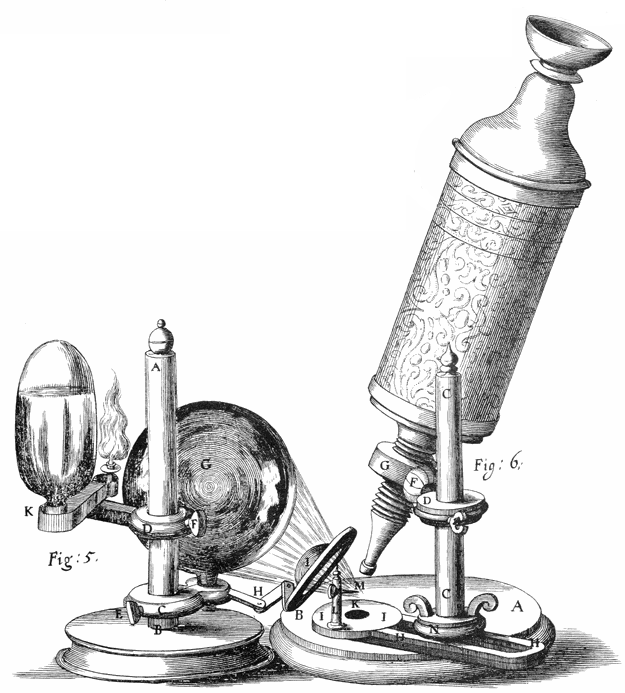
\includegraphics[scale=.15]{Hooke_microscope.png}\vspc
		\includegraphics[scale=.3]{Hooke_Signature.png}
			
		\begin{itemize}
		    \item Mechanics
		    \item Gravitation
		    \item Horology
		    \item Microscopy
		    \item Palaeontology
		    \item Astronomy
		    \item Memory
		\end{itemize}
		
		
		\end{multicols}
		
		\vspace{1mm}
		{\tiny Images: \href{https://en.wikipedia.org/wiki/Robert_Hooke}{Wikipedia}}
	}
	
	% Section I - Frame I
	\frame{
		\frametitle{\sectiontitleI}
		
		\small
		Robert Hooke FRS (...1635 ...1703) was an English natural philosopher, architect and polymath. As a young adult, he was a financially impoverished scientific inquirer, but came into wealth and good reputation following his actions as Surveyor to the City of London after the great fire of 1666 (in which he appears to have performed more than half of all the surveys after the fire). At that time, he was also the curator of experiments of the Royal Society, a member of its council, and the Gresham Professor of Geometry. He was also an important architect of his time—though few of his buildings now survive and some of those are generally misattributed—and was instrumental in devising a set of planning controls for London, the influence of which remains today. Allan Chapman has characterised him as "England's Leonardo".[1]
		
		{\tiny Text: \href{https://en.wikipedia.org/wiki/Robert_Hooke}{Wikipedia}}
	}

% Section II
\section{\sectiontitleII}
	
	% Section II - Frame I
	\frame{
		\frametitle{\sectiontitleII}
		\vspace{3mm}
		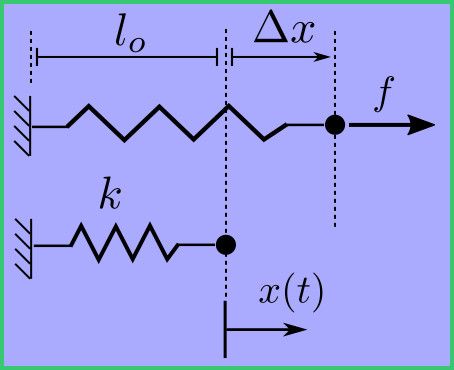
\includegraphics[scale=.35]{hookes_law_fig1.png}\hspace{10mm}		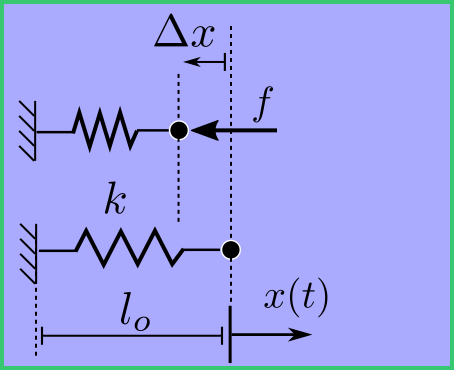
\includegraphics[scale=.35]{hookes_law_fig2.png} \vspc
		
		The simple and effective model of spring behavior is called the {\PR linear force-deflection model}. \vspc
		
		\begin{framed}
		\scalebox{1}{$f = kx$} \hspc , \hspc {\it force equals spring constant times deflection} \vspc
		\end{framed}
		
		\vspace{1mm}
		{\tiny Images: T. Hill }
	}
	
	
	% Section II - Frame II
	\frame{ 
		\frametitle{\sectiontitleII}
		
		\begin{multicols}{2}
		
		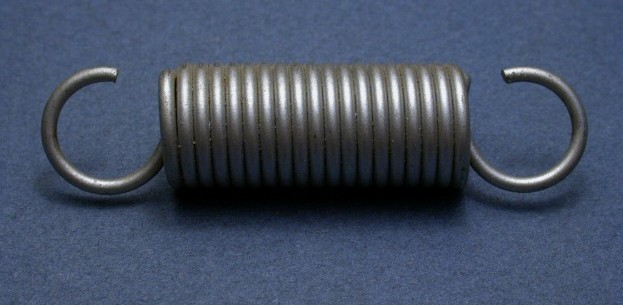
\includegraphics[scale=.35]{coil_spring.jpg} \hspc \scalebox{1}{$k = \frac{Gd^4}{64nR^3}$} \vspc
		
		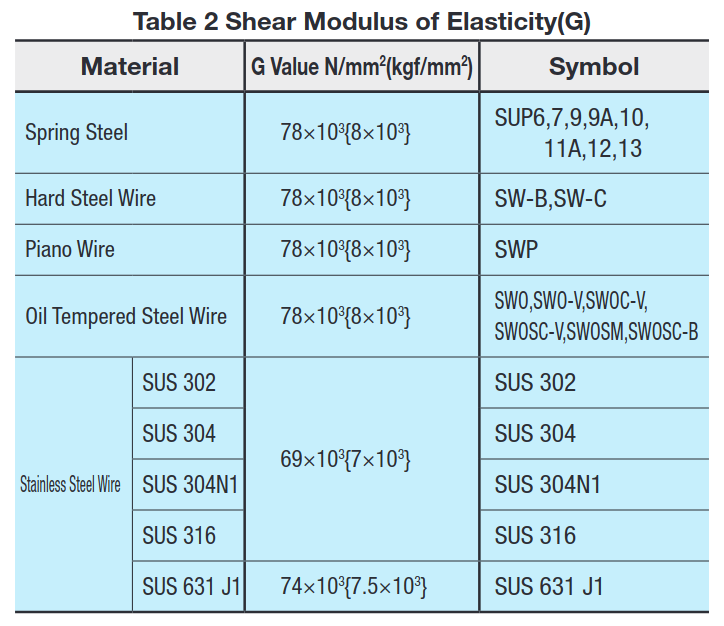
\includegraphics[scale=.2]{shear_modulus.png} \vspc
		
		\vspace{1mm}
		{\tiny Data: \href{https://us.misumi-ec.com/pdf/tech/mech/US2010_fa_p3501_3502.pdf}{MISUMI} }
		\vspace{2mm}

		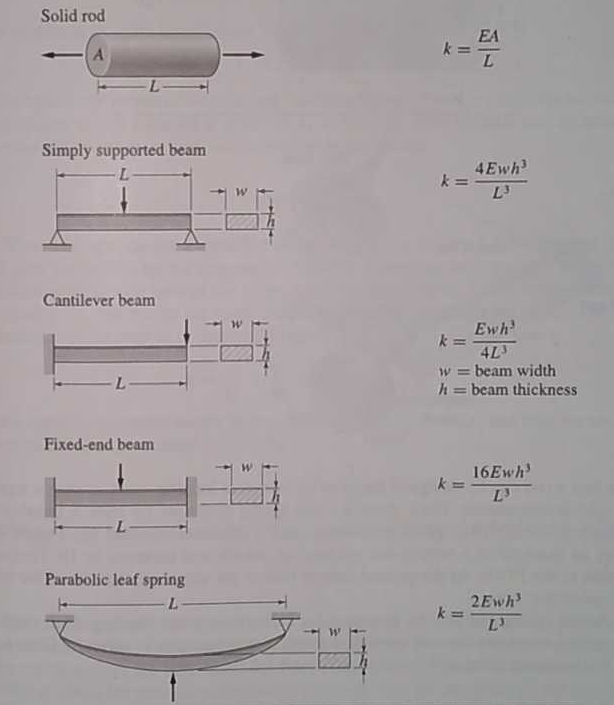
\includegraphics[scale=.22]{types_of_springs.png}
		\vspace{2mm}
		{\tiny Images:  Wikipedia, System Dynamics}		
		
		\end{multicols}
	
	}

% Section III
\section{\sectiontitleIII}
	
	% Section III - Frame I
	\frame{
		\frametitle{\sectiontitleIII}
		
		The ideal {\PR linear force-deflection model} is only an approximation of the true behavior. However, homogeneous isotropic materials do behave this way in the {\it linear elastic region}. \vspc
		
		%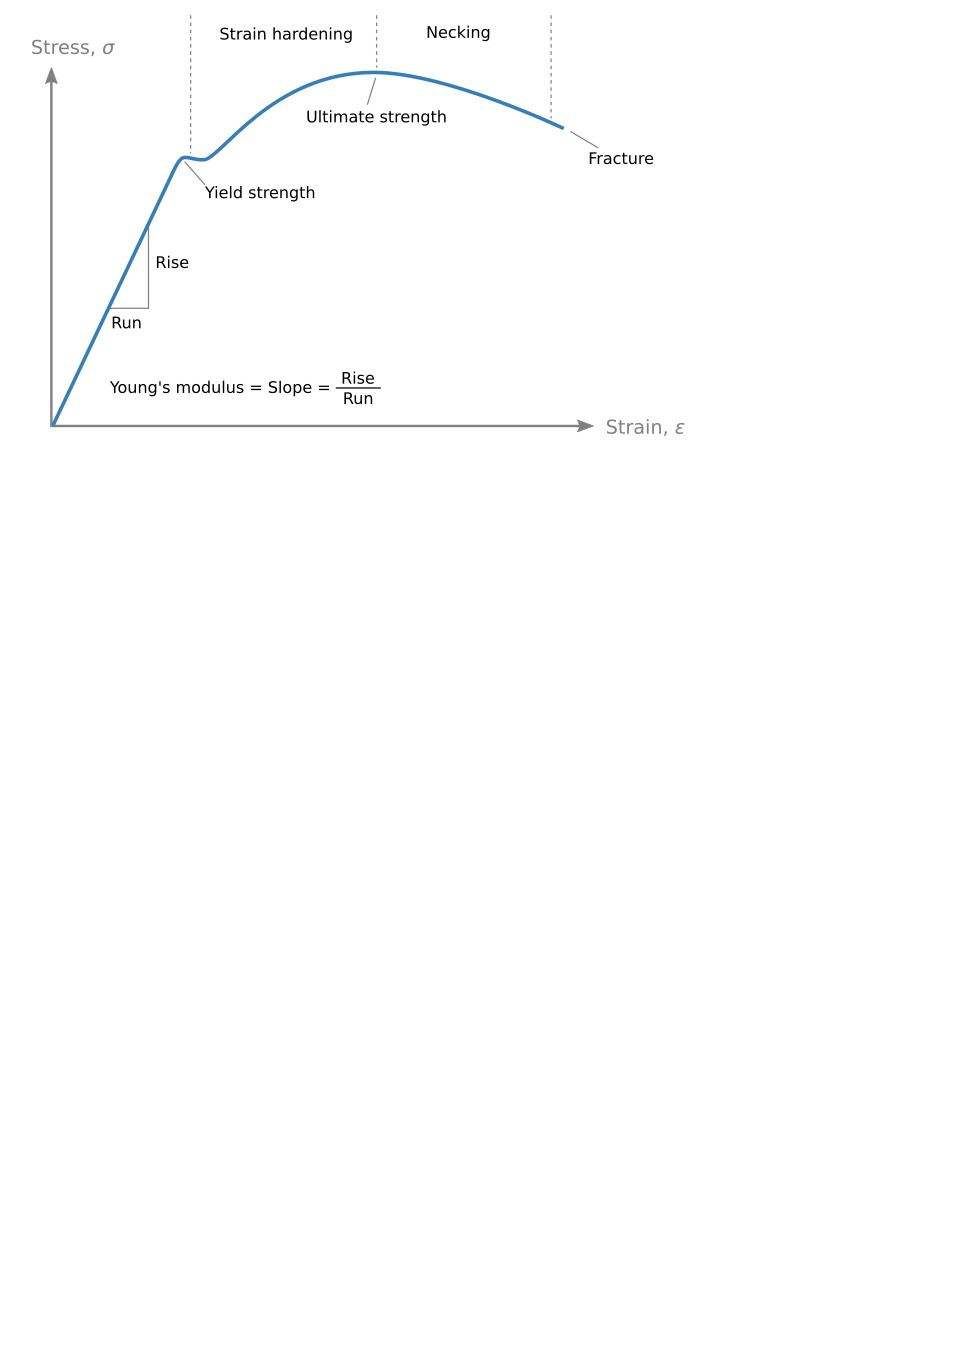
\includegraphics[scale=.3]{stress_strain_fig1.png} \scalebox{1}{$\rightarrow$} %
		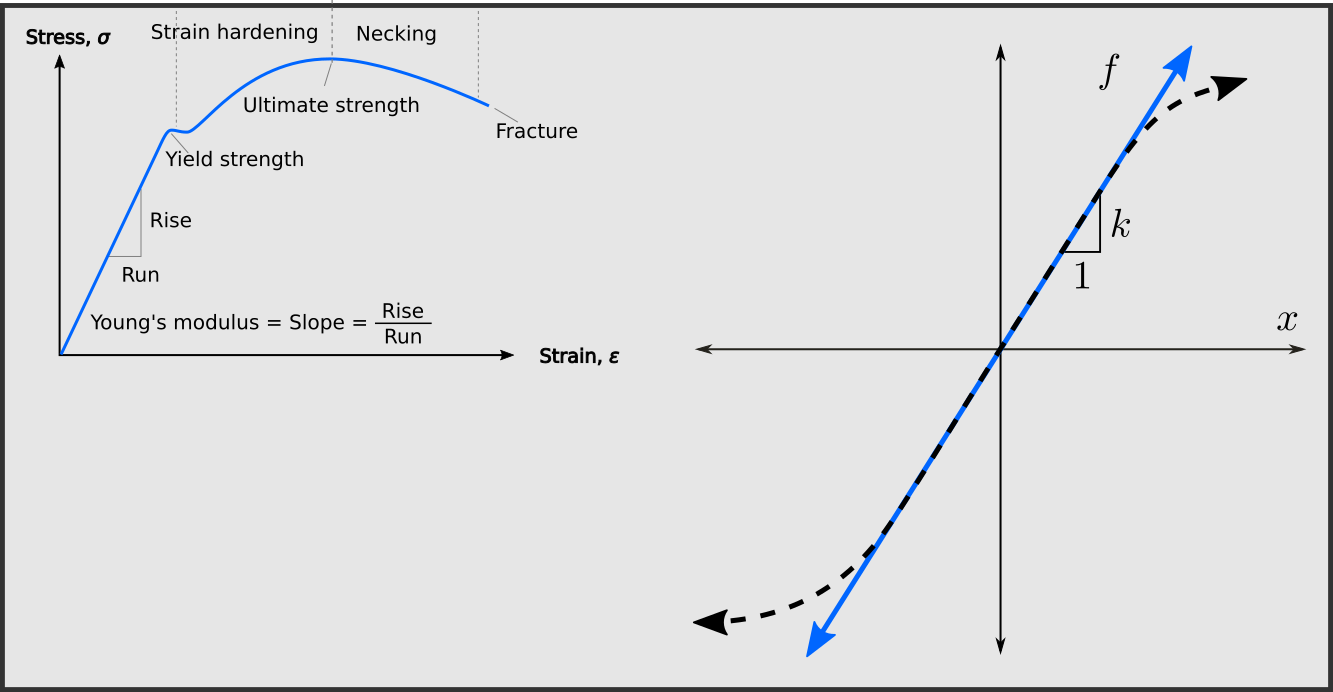
\includegraphics[scale=.2]{nonlinear_spring.png}
		
		\vspace{1mm}
		{\tiny Images: T. Hill }
		}
		
% Section IV:
\section{\sectiontitleIV}

	% Section IV - Frame I
	\frame{
		\frametitle{\sectiontitleIV}
	
		All physical structures deform under load, and as we know, every force as reaction force. Therefore any structure {\it acts} like a spring under load.  
	
	}
	
\end{document}





